\documentclass{article}
\usepackage[francais]{babel}
\usepackage[utf8]{inputenc}
\usepackage{xcolor}
\usepackage[pdftex]{graphicx}
\usepackage{listings}
\usepackage{amsmath}
\usepackage[a4paper,includeheadfoot,margin=2.54cm]{geometry}
\usepackage{amsfonts}
\usepackage{fancyhdr}
\usepackage{titling}
\usepackage{algorithm}
\usepackage{algpseudocode}
\usepackage{hyperref}

\pagestyle{fancy}
\fancyhf{}
\fancyhead[LE,RO]{\theauthor}
\fancyhead[RE,LO]{\thetitle}
\fancyfoot[CE,CO]{\leftmark}
\fancyfoot[LE,RO]{\thepage}

%Syntax coloring C
\definecolor{mGreen}{rgb}{0,0.6,0}
\definecolor{mGray}{rgb}{0.5,0.5,0.5}
\definecolor{mPurple}{rgb}{0.58,0,0.82}
\definecolor{backgroundColour}{rgb}{1,1,1}

\lstdefinestyle{CStyle}{,
    backgroundcolor=\color{backgroundColour},   
    commentstyle=\color{mPurple},
    keywordstyle=\color{mGreen},
	identifierstyle=\color{blue},
    numberstyle=\tiny\color{mGray},
    stringstyle=\color{orange},
    basicstyle=\footnotesize,
    breakatwhitespace=false,         
    breaklines=true,                 
    captionpos=b,                    
    keepspaces=true,                 
    numbers=left,                    
    numbersep=5pt,                  
    showspaces=false,                
    showstringspaces=false,
    showtabs=false,                  
    tabsize=2,
    language=C
}
\usepackage[thinlines]{easytable}

\title{Rapport de TP : Alignement optimal et détection de plagiat}
\author{Annie LIM, Quentin GARRIDO}
\date{6 janvier 2020}

\begin{document}

\maketitle
\tableofcontents
\pagebreak

\section{Introduction}

Ce TP a pour but de concevoir un logiciel d'aide à la détection de plagiat.\\
Ce logiciel d'alignement de séquences affichera simultanément le texte que l'on pense être du plagiat avec le texte original, en mettant en avant les correspondances. Moins les textes diffèrent et plus les chances de détecter un plagiat sont grandes.\\

%==============================================================================
\section{Exercice 1}

Pour calculer le score d'un alignement optimal entre x et y, nous pouvons utiliser l'algorithme de distance de Levenshtein, appelé distance d'édition (edit distance).\\
Nous voulons observer les différences entre deux textes. Cela revient à calculer leur score d'alignement, le coût des opérations nécessaires (deletion, insertion, substitution) pour obtenir le même texte. Plus ce score est faible et plus les textes sont similaires, et donc sujet d'être un plagiat.\\
Le score optimal correspond au minimum entre les trois valeurs données par les opérations deletion, insertion et substitution. \\
Algo...\\
Cet algorithme est bien de complexité $O(\lvert x\rvert \times \lvert y\rvert)$.


%==============================================================================
\section{Exercice 2}

Soit une matrice T telle que $T[i][j]$ est le score d'un alignement optimal entre $x_{i}$ et $y_{j}$ avec $x_{i}$ ry $y_{j}$ les préfixes de x et y de longueur i et j.\\
A partir de cette matrice, nous pourrons retrouver les opérations nécessaires à la solution optimale pour aligner les deux textes, afin de construire les textes 1 et 2 modifiés alignés.\\
Le backtracking consiste à suivre le chemin minimum de la matrice T de
$T[i][j]$ jusqu'à $T[0][0]$.\\
Algo...\\
Cet algorithme est bien de complexité $O(\lvert x\rvert+\lvert y\rvert)$.

%==============================================================================
\section{Exercice 3}


%==============================================================================
\section{Exercice 4}
\subsection{Théorie}
\subsubsection{Algorithme}
Le principal changement ici est que nous voulons mettre en correspondance des
lignes entre elles (séparées par des \textbackslash{}n).\\
Précédemment nous alignions un texte composé de caractères, mais maintenant nous
voulons aligner un texte composé de lignes/phrases/paragraphes qui seront nos
éléments de "base".\\

Le problème étant très similaire au précédent, la méthode que nous utilisions
devrait pouvoir être adaptée à ce nouveau problème.\\
Pour ce faire nous allons définir une nouvelle distance de Levenshtein agissant sur
des lignes entières et plus uniquement des caractères.
Nous allons définir la substitution, insertion, et délétion comme suit:

\begin{gather*}
	\text{Ins'}(y) = Lev(\epsilon,y) = \lvert y \rvert\\
	\text{Del'}(x) = Lev(x,\epsilon) = \lvert x \rvert\\
	\text{Sub'}(x,y) = Lev(x,y)
\end{gather*}
Ici Lev(x,y) est la distance de levenshtein définie précédemment, et x et y
sont des lignes.\\

Il est assez facile de voir pourquoi nous avons choisi comme coût d'insertion
et de délétion la longueur du paragraphe. En effet cela correspond à ajouter
(resp. enlever) les caractères un par un, avec un coût de 1 à chaque fois.\\

Pour la substitution il est un peu moins clair au premier abord sur quelle
valeur choisir. Le choix le plus simple est de supprimer puis d'insérer les
paragraphes, cependant ce ne serait pas une distance car dans ce cas là
$Sub(x,x) \neq 0$.\\
Nous avons étudié plusieurs distances entre les textes, chacunes avec leur
défauts et avantages, mais celle qui paraît la meilleure est la distance de
Levenshtein, qui nous donnera une meilleure indication de la différence entre
nos paragraphes, et nous permettra ensuite facilement de créer un alignement
ayant du sens.\\
Puisque nous avons considéré un coût d'ajout et de suppresion d'un caractère de
1 pour définir $Sub'$ et $Ins'$ nous devons faire pareil dans la distance de
Levenshtein, et nous considérerons un coût de substitution de 1 si les
caractères dont différents et 0 sinon.\\

Nous pouvons ensuite définir notre nouvelle distance de Levenshtein comme suit:
\begin{equation*}
	Lev'(x.a,y.b)= min
		\begin{cases}
			Lev'(x.a,y) + Ins'(b)\\
			Lev'(x,y.b) + Del'(a)\\
			Lev'(x,y) + Sub'(a,b)
		\end{cases}
		= min
		\begin{cases}
			Lev'(x.a,y) + \lvert b \rvert\\
			Lev'(x,y.b) + \lvert a \rvert\\
			Lev'(x,y) + Lev(a,b)
		\end{cases}
\end{equation*}
Ici $a$ et $b$ ne sont plus des caractères mais sont désormais des
paragraphes.\\
Nous sommes donc en mesure d'adapter le code précédemment écrit pour cette
nouvelle version, sans faire beaucoup de changements.\\

Nous pouvons nous demander si $Lev'$ est toujours une distance.\\
Étant donné que $Lev$ est une distance et aue $Sub'(x)=Ins'(x)$ nous pouvons
conclure que nous avons bien une distance.\\


Pour l'algorithme de construction de l'alignement optimal, il est identique à
celui vu précédemment, en adaptant juste la reconstruction des paragraphes.\\
Si nous avons choisi $Ins'$ ou $Del'$ nous construisons une chaine de caractère
vide.\\
Si nous avons choisi $Sub'$ nous construsions l'alignement optimal entre nos
deux paragraphes comme nous l'avons fait précédemment.

\subsubsection{Complexité}

L'algorithme va remplir $n \times m$ cases (n et m étant le nombre de
paragraphes des textes que nous souhaitons aligner).\\
Il faut donc trouver la complexité de $Lev'$ afin de conclure sur la complexité
totale.\\
Les complexités des différentes opérations sont:
\begin{itemize}
	\item $Lev'(x.a,y) + \lvert b \rvert$ a une complexité en $O(\lvert b
		\rvert)$ dans le pire des cas (comme \textit{strlen} en C) 
	\item $Lev'(x,y.b) + \lvert a \rvert$ a une complexité en $O(\lvert a
		\rvert)$ dans le pire des cas (comme \textit{strlen} en C) 
	\item $Lev'(x,y) + Lev(a,b)$ a une complexité en $O( \lvert a \rvert \times
		\lvert b \rvert)$
\end{itemize}

Si nous notons $l$ la longueur du plus long paragraphe, la complexité de calcul
de $Lev'$ est alors $O(l^2+l+l) = O(l^2)$.\\
La complexité totale du calcul de la table est donc $O(m \times n \times l^2)$.\\

Nous avons vu la complexité pour calculer la table des ditances, regardons
maintenant pour la construction de l' alignement optimal.\\
Pour aligner deux paragraphes, si nous avons gardé en mémoire les tables des
distances de Levenshtein utilisées pour le calcul de $Sub'$ lors de la
construction de la table de $Lev'$ la complexité sera de $O(l)$.\\
Si en revanche nous ne les avons pas gardé en mémoire (comme dans notre
implémentation) la complexité sera alors de $O(l^2)$ pour reconstruire la table
puis $O(l)$ pour construire l' alignement dans le cas où l' opération choisie
est la substitution. Dans ce cas, la complexité de la construction de
l'alignement de deux paragraphes est $O(l^2)$ si nous avons choisi la
substitution et $O(l)$ sinon. Il serait alors intéressant en cas d'égalité de
choisir l'opération la moins coûteuse.

Nous obtenons alors une complexité totale pour la construction de l'alignement 
des textes de $O((m+n)\times l^2)$ si nous n'avons pas gardé les tables en
mémoire et et de $O((m+n)\times l)$ si nous l'avons fait.


\subsection{Implémentation}

L'implémentation pour le calcul de la table est presque identique à celle de
l'exercice 3, nous avons juste changé le calcul de sub, ins et del.\\
Le code est disponible en annexe des lignes 324 à 373.\\
Afin de séparer les différents paragraphes des textes, nous avons implémenté
une fonction utilisant \textit{strtok\_r} qui devrait donc être compatible sur tous les
OS, qu'ils respectent les normes POSIX ou non.\\
Son implémentation est fournie en annexe aux lignes 307 à 322.\\

Pour le backtracking aussi le principe reste le même.\\
Pour l'alignement si nous avons fait une insertion ou délétion nous allons
implement insérer une chaîne remplie du caractère vide de bonne longueur.\\
Si nous avons fait une substitution nous allons alors insérer l'alignement
entre les deux textes substitués.\\
Le code est disponible en annexe des lignes 375 à 439.\\

\begin{figure}[!hbt]
	\centering
	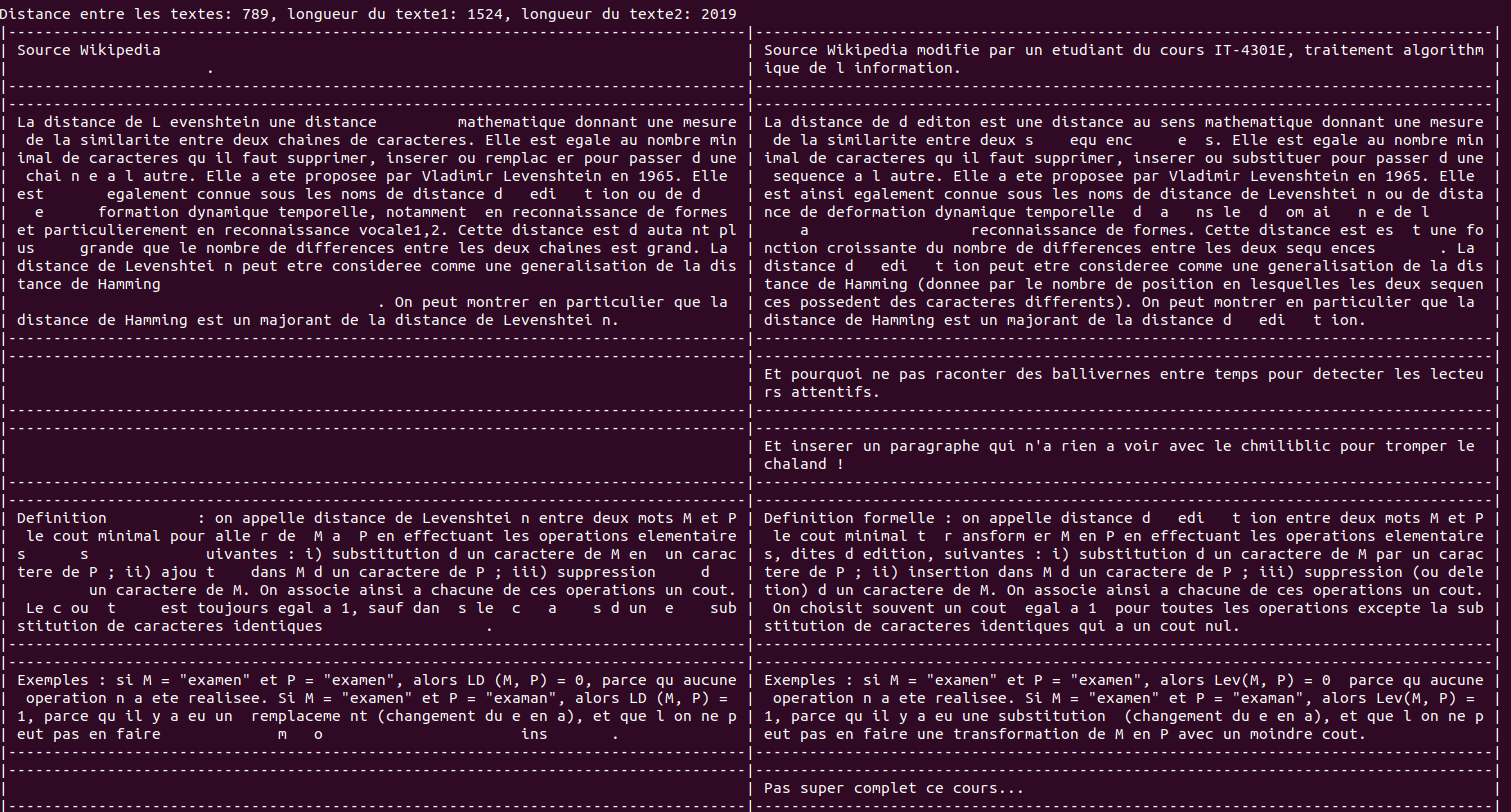
\includegraphics[width=0.95\linewidth]{./images/exo4.png}
	\caption{Résultat de l'alignement des textes paragraphe par paragraphe}%
	\label{fig:exo4}
\end{figure}

Comme nous pouvons le voir sur la figure~\ref{fig:exo4}, nous obtenons bien un
bon alignement des deux textes, identique au résultat attendu, à quelques
détails d'affichage près.\\

D'après les tests et vérifications que nous avons effectuées avec Valgrind, le
programme ne comporte aucune fuite mémoire.\\


\clearpage
%=============================================================================
\section{Annexe: Code source}
		\lstinputlisting[label=code,style=CStyle]{../TD2.c}

\end{document}
